\documentclass[tikz,border=2pt]{standalone}
\usepackage{amsmath,amssymb}
\usepackage{tikz}
\usetikzlibrary{matrix,arrows.meta}

\begin{document}
% A forbidden pair (agent 2 may not do task 3) gets cost infinity; row and column reductions
% leave it infinite, so it can never become a zero and is never selected.
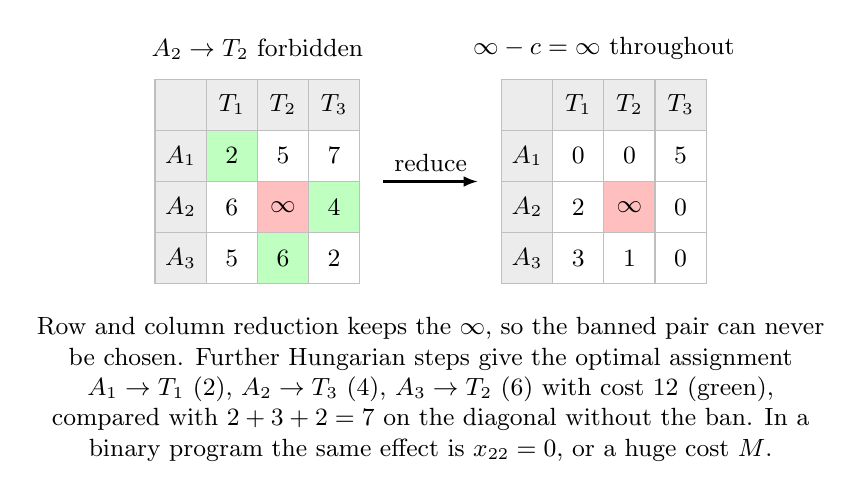
\begin{tikzpicture}[every node/.style={font=\small}, >={Latex[length=1.8mm]}]
	\matrix (A) [matrix of math nodes, nodes={minimum size=6.5mm, anchor=center, draw=gray!50}, column sep=-\pgflinewidth, row sep=-\pgflinewidth] at (0,0) {|[fill=gray!15]| & |[fill=gray!15]| T_1 & |[fill=gray!15]| T_2 & |[fill=gray!15]| T_3 \\ |[fill=gray!15]| A_1 & |[fill=green!25]| 2 & 5 & 7 \\ |[fill=gray!15]| A_2 & 6 & |[fill=red!25]| \infty & |[fill=green!25]| 4 \\ |[fill=gray!15]| A_3 & 5 & |[fill=green!25]| 6 & 2 \\};
	\node[anchor=south] at (A.north) {$A_2\to T_2$ forbidden};
	\draw[->, thick] (1.6,0) -- (2.8,0) node[midway, above] {reduce};
	\matrix (B) [matrix of math nodes, nodes={minimum size=6.5mm, anchor=center, draw=gray!50}, column sep=-\pgflinewidth, row sep=-\pgflinewidth] at (4.4,0) {|[fill=gray!15]| & |[fill=gray!15]| T_1 & |[fill=gray!15]| T_2 & |[fill=gray!15]| T_3 \\ |[fill=gray!15]| A_1 & 0 & 0 & 5 \\ |[fill=gray!15]| A_2 & 2 & |[fill=red!25]| \infty & 0 \\ |[fill=gray!15]| A_3 & 3 & 1 & 0 \\};
	\node[anchor=south] at (B.north) {$\infty-c=\infty$ throughout};
	\node[anchor=north, align=flush center, text width=10cm] at (2.2,-1.6) {Row and column reduction keeps the $\infty$, so the banned pair can never be chosen. Further Hungarian steps give the optimal assignment $A_1\to T_1$ ($2$), $A_2\to T_3$ ($4$), $A_3\to T_2$ ($6$) with cost $12$ (green), compared with $2+3+2=7$ on the diagonal without the ban. In a binary program the same effect is $x_{22}=0$, or a huge cost $M$.};
\end{tikzpicture}
\end{document}
